% !TeX root = ..\main.tex
\pagestyle{fancy-style}
\npchapter{Einleitung} \label{introduction}
\pagenumbering{arabic}
Dieses Kapitel führt in die Thematik ein und motiviert, warum Bun evaluiert werden soll. Darauf werden die Ziele und der Aufbau dieser Arbeit vorgestellt.

\section{Motivation} \label{sec:introduction-motivation}
Die kontinuierliche Evolution von Softwaretechnologien und -umgebungen hat einen erheblichen Einfluss auf die Entwicklung und Leistung von Anwendungen. Kürzlich wurde die Version 1.0 der JavaScript Laufzeitumgebung Bun veröffentlicht, die vielversprechende Verbesserungen in Bezug auf die Leistung im Vergleich zu Node.js ankündigt \cite{Sumner.2023}. \newline
JavaScript ist eine Programmiersprache, die vor allem im Kontext der Web-Entwicklung verwendet wird \cite{Brown.November2019}. Aktuell erfreut sich JavaScript großer Beliebtheit. In einer Umfrage unter Entwicklern auf Stack Overflow, an der mehr als 89.000 Entwickler teilgenommen haben, wurde JavaScript zum 11. Jahr in Folge als die am häufigsten verwendete Programmiersprache identifiziert. Mehr als 63\% der befragten Entwickler haben JavaScript als ihre favorisierte Technologie angegeben. Unter den professionellen Entwicklern liegt der Anteil noch höher, bei mehr als 65\%. Zusätzlich ist TypeScript, eine stark typisierte Programmiersprache, die auf 
JavaScript aufbaut, ebenfalls beliebt \cite{Microsoft.o.J.}. Etwa 39\% aller Entwickler und ungefähr 44\% der professionellen Entwickler nutzen TypeScript. Somit ist TypeScript die viertbeliebteste Programmiersprache. \cite{StackOverflow.2023} Dies unterstreicht die hohe Relevanz des JavaScript-Ökosystems.\\

\begin{figure}[h]
	\centering
	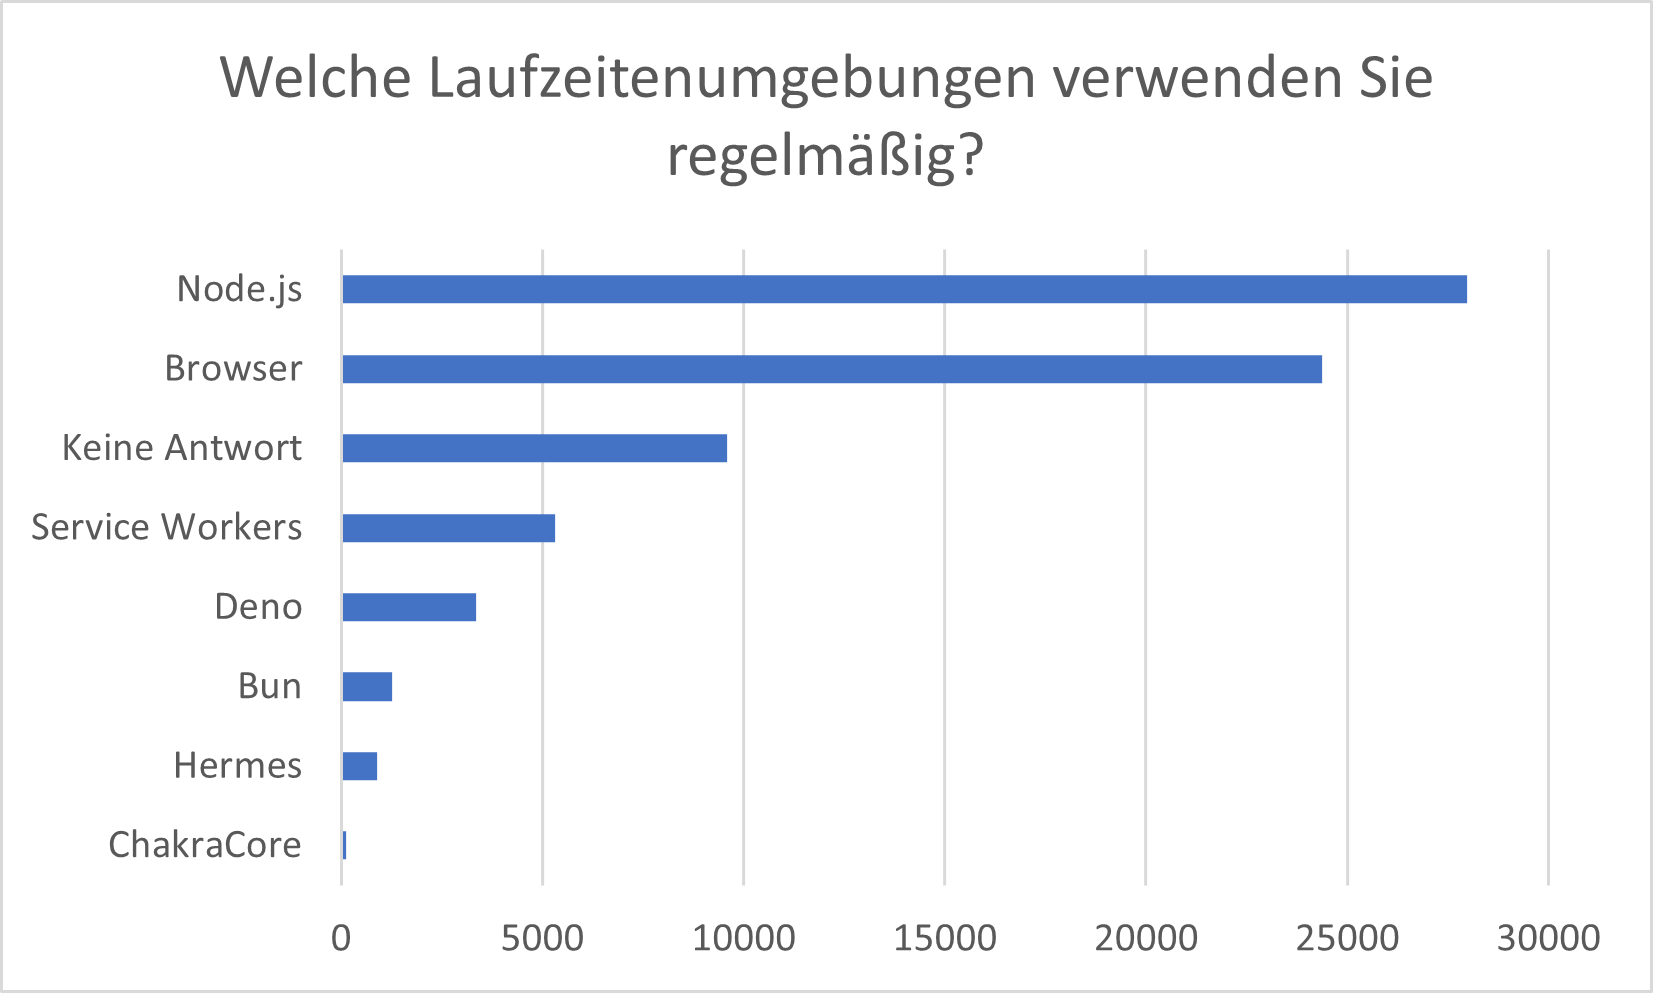
\includegraphics[width=\linewidth]{./images/WhichRuntimesDoYouUseRegularly}
	\caption{Nutzungsstatistik von JavaScript-Laufzeitumgebungen \cite{Greif.2022}}
	\label{fig:runtime-share}
\end{figure}

\noindent
JavaScript wird nicht nur für die Entwicklung im Frontend, sondern auch für die Entwicklung im Backend 
eingesetzt. Etwa 3\% der weltweit bekannten Server nutzen eine Laufzeitumgebung, die JavaScript 
ausführen kann. \cite{QSuccess.2023} Wie aus Abbildung \ref{fig:runtime-share} ersichtlich ist, ist Node.js die am weitesten verbreitete Laufzeitumgebung. In der Umfrage zur aktuellen Verwendung von JavaScript gaben ca. 71\% der 30.000 befragten Entwickler an, dass sie Node.js regelmäßig als Laufzeitumgebung verwenden.
Lediglich ca. 9\% der befragten Entwickler verwenden Deno, während ungefähr 3\% Bun als eine Alternative zu Node.js benutzen. \cite{Greif.2022}


\section{Zielsetzung} \label{sec:introduction-target}
Aktuell ist Node.js die am weitesten verbreitete Laufzeitumgebung für JavaScript. Dennoch erscheinen immer wieder neue Laufzeitumgebungen, die versuchen, Node.js zu verdrängen. Eine neue Alternative ist Bun, das am 9. September 2023 in der Version 1.0 veröffentlicht wurde. Die Entwickler von Bun werben mit Features wie erheblicher Leistungssteigerung, eleganten Schnittstellen und einer angenehmen Entwicklererfahrung. \cite{Sumner.2023}\\

\noindent
Das Hauptziel dieser Arbeit besteht darin, die Version 1.0 von Bun einer eingehenden Evaluierung zu unterziehen. Konkret wird untersucht, ob die in den Ankündigungen versprochene signifikante Leistungssteigerung im Vergleich zu Node.js tatsächlich existiert und reproduzierbar ist. Darüber hinaus wird geprüft, inwiefern bestehende Projekte auf der Basis von Node.js mit Bun kompatibel sind. Die Ergebnisse dieser Arbeit können Entwicklern bei der Entscheidung helfen, ob sie auf Bun 1.0 migrieren sollten, und sie dabei unterstützen, die Leistung ihrer bestehenden Projekte zu verbessern. Insgesamt zielt diese Untersuchung darauf ab, Klarheit über die Versprechungen von Bun 1.0 zu schaffen und Entwicklern fundierte Informationen für ihre Entscheidungsfindung zur Verfügung zu stellen. Dies spiegelt sich in den folgenden Leitfragen wider:
\begin{itemize}
    \item Welche konkreten Leistungsverbesserungen können in Bun 1.0 im Vergleich zu Node.js festgestellt werden, und wie lassen sie sich quantifizieren?
    \item Inwiefern sind Node.js-Projekte kompatibel mit Bun? Wie schwierig gestaltet sich die Migration?
    \item Welche Herausforderungen und potenziellen Vorteile ergeben sich bei der Verwendung von Bun 1.0 im Vergleich zu Node.js für Entwickler und Projekte?
\end{itemize}

\section{Aufbau der Arbeit} \label{sec:introduction-overview}
Im folgenden Kapitel vermittelt die Arbeit alle notwendigen theoretischen Grundlagen, die zum Verständnis des Themas notwendig sind. Dafür werden Node.js und Bun detailliert betrachtet. Des Weiteren wird Performance als Qualitätsattribut von Software definiert, um Rückschlüsse für die Performance-Analyse zu ermöglichen.\\

\noindent
Im dritten Kapitel werden die Performance von Bun und Node.js in ausgewählten Testszenarien verglichen. Hierzu werden zuerst die Vorgehensweise, der Versuchsaufbau und die Implementierungen vorgestellt. Im Anschluss daran folgt de die Präsentation der Ergebnisse und ein zusammenfassendes Fazit.\\

\noindent
Das vierte Kapitel setzt den Fokus auf die Kompatibilität von Projekten auf Basis von Node.js. Der Fokus liegt auf den Frameworks Express und NestJS. Um die Kompatibilität bewerten zu können, werden 2 Anwendungen beispielhaft migriert. Die Ergebnisse werden in einem Fazit eingeschätzt.\\

\noindent
Das letzte Kapitel fasst die Kernaussagen der Arbeit zusammen und prüft sie vor dem Hintergrund der zuvor definierten Ziele. Abschließend wird in einem Ausblick dargelegt, welche ergänzenden Forschungsthemen verbleiben und welchen zukünftigen Nutzen die Ergebnisse mit sich bringen.


